\documentclass[nostrict]{szablonPG}

%-------------------- Dodatkowe pakiety ---------------------
\usepackage{listing_schemat}
%------------------------------------------------------------

%------------------------------------------------------------
%			      Pocz�tek pracy dyplomowej  
%------------------------------------------------------------

\begin{document}

%------------------------------------------------------------
%	Utworzenie spisu tre�ci 
\tableofcontents

%------------------------------------------------------------
%	Dodanie rozdzia��w 

\chapter{Kr�tka instrukcja obs�ugi}

\begin{flushright}
  \small{
        \parbox{8cm}{
                {\small
                        \textit{Do what you think is interesting,
                        do something that you think is fun and worthwhile,
                        because otherwise you won't do it well anyway.}
                }
                \vspace{.5cm}\hfill{---Brian W. Kernighan}
        }
 }
\end{flushright}

Pakiet \verb|SzablonPG| powsta�, aby u�atwi� pisanie prac dyplomowych na Politechnice Gda�skiej. U�atwienie to ma polega� na podaniu
szablonu \LaTeX'owego pracy dyplomowej, kt�ry b�dzie maksymalnie zgodny z wytycznymi dla autor�w
podanych w Zarz�dzeniu Rektora 22/2018 z 20 czerwca 2018 roku. W ten spos�b zamiast ,,walczy�'' z \LaTeX'em lub stara� si�
z�o�y� prac� w MS Word mo�na skupi� si� na tre�ci. Korzystanie z \LaTeX'a szczeg�lnie w przypadku prac
matematycznych wydaje si� by� wskazane z uwagi na �atwo�� sk�adania i jako�� z�o�onych formu�
matematycznych.


\section{Jak u�y� szablonu}

Szablon dostarcza klasy \verb|SzablonPG|, kt�r� nale�y u�y� zamiast standardowych klas np.:
\verb|article|, \verb|report|. Plik \verb|szablonPG.cls| \textbf{musi by�} umieszczony w tym samym
katalogu, co g��wny plik pracy. Na pocz�tku g��wnego pliku pracy piszemy
\begin{verbatim}
    \documentclass{szablonPG}   % zamiast standardowych klas np.: article
\end{verbatim}
Plik \verb|SzablonPracyPG_main.tex| pokazuje jak mo�e wygl�da� praca z�o�ona z u�yciem tej klasy.

\section{Pisanie w \LaTeX'u}

Aby wygodnie pisa� w \LaTeX'u potrzebujemy:
\begin{enumerate}
 \item dystrybucji \TeX'a np.: MikTeX lub TeXLive (Linux)
 \item edytora np.: LED, WinEdit, Kile (Linux)
\end{enumerate}

Podstawowym �r�d�em wiedzy o programowaniu jest dostarczana z ka�d� dystrybucj� dokumentacja:
\begin{enumerate}
 \item A Gentle Introduction to TEX,
 \item The Not So Short Introduction to LATEX
\end{enumerate}

Internet jest pe�en wprowadze�, tutoriali i przyk�ad�w. Nieocenionym �r�d�em wiedzy s� strony:
\begin{verbatim}
http://google.com/
http://faq.gust.org.pl/
http://tex.stackexchange.com/
\end{verbatim}

\section{Organizacja projektu}

Pisanie w jednym pliku du�ego projektu, powoduje, �e w pewnym momencie ci�ko odszuka� w�r�d setek
linii kodu t� w�a�ciw�. System \LaTeX umo�liwia podzielenie kodu �r�d�owego na osobne pliki, s�u��
do tego polecenia \verb|\input| oraz \verb|\include|. Opiszemy spos�b korzystania z tego drugiego
polecenia.

Na pocz�tek dzielimy nasz� prac� na logiczne fragmenty. W przypadku pracy dyplomowej mog� to by�
np.: rozdzia�y. Nast�pnie tworzymy osobne pliki \TeX'owe dla ka�dego rozdzia�u i~jeden plik g��wny.

W pliku g��wnym umieszczamy wszystkie deklaracje, do��czamy pakiety, kt�rych chcemy u�y� i sekwencj�
\verb|\begin{document} ... \end{document}|. W tej sekwencji za pomoc� polecenia \verb|\include|
do��czamy pliki rozdzia��w. W plikach rozdzia��w piszemy \textbf{tylko kod rozdzia�u}.

Za��my, �e nasza praca sk�ada si� ze \textit{Wst�pu, Rozdzia�u 1 i Rozdzia�u 2}. Tworzymy wtedy
pliki (nazwy plik�w przyk�adowe): \verb|praca_glowny.tex|, \verb|praca_wstep.tex|,
\verb|praca_rozdzial1.tex|, \verb|praca_rozdzial2.tex|. UWAGA! \LaTeX\ nie lubi spacji w nazwach
plik�w. Przyk�adowo, pliki mog�yby wygl�da� tak:
\begin{multicols}{2}
\begin{verbatim}
% praca_glowny.tex
\documentclass{SzablonPracyPG}
%inne pakiety, definicje itp.
\begin{document}
\tableofcontents
  \include{praca_wstep}
  \include{praca_rozdzial1}
  \include{praca_rozdzial2}
% bibilografia etc.
\end{document}
%EOF
\end{verbatim}
\columnbreak
\begin{verbatim}
% praca_wstep.tex
\chapter*{Wst�p}

To jest wst�p.
\end{verbatim}
\begin{verbatim}
% praca_rozdzial1.tex
\chapter{Tytu� pierwszego rozdzia�u}

Tre�c pierwszego rozdzia�u.
\end{verbatim}
\begin{verbatim}
% praca_rozdzial2.tex
\chapter{Tytu� drugie rozdzia�u}

Tre�� drugiego rozdzia�u.
\end{verbatim}
\end{multicols}

Pliki nie musz� by� umieszczone w tym samy katalogu co plik g��wny, trzeba wtedy poprzedzi�
nazw� pliku �cie�k� do katalogu w kt�rym znajduje si� plik. Przyk�adowo mo�na w tym celu u�y� nast�puj�cego polecenia: \verb|\input{rozdzialy/praca_rozdzial1.tex|. Wszystkie edytory \TeX'owe wspieraj�
tworzenie projekt�w, czyli prace w ten spos�b, pomagaj�c w ten spos�b zapanowa� nad struktur� pracy.
Dla d�ugich projekt�w przydatne jest tak�e polecenie \verb|\includeonly|. 

\section{Strona tytu�owa i o�wiadczenie}


Najpro�ciej - umieszczamy w katalogu \textbf{meta} pliki o�wiadczenia oraz strony tytu�owej wygenerowane z serwisu MojaPG, zapisane po uzupe�nieniu danych w formacie pdf. Nast�pnie w g��wnym pliku pracy dyplomowej dodajemy pliki do ca�ego dokumentu przy u�yciu polece�:
\begin{verbatim}
%------------------------------------------------------------
%  Dodanie strony tytu�owej wygenerowanej z MojaPG oraz 
%  						o�wiadczenia
\includepdf{meta/strona_tytulowa.pdf}
\includepdf{meta/oswiadczenie.pdf}
%------------------------------------------------------------
\end{verbatim}

Polecenia te znajduj� si� ju� w przyk�adowym pliku g��wnym pracy \verb|SzablonPracyPG_main.tex|.

\section{J�zyk polski i kodowanie}

W przypadku, gdy:
\begin{enumerate}
 \item plik \verb|SzablonPracyPG_main.tex| nie chce si� kompilowa�,
 \item kod �r�d�owy tego przyk�adu zawiera ,,krzaczki'',
 \item widoczny po skompilowaniu tekst: nie zawiera polskich liter,
 \item zamiast polskich liter wy�wietla ,,krzaczki'',
\end{enumerate}
to jedn� z przyczyn mo�e by� niew�a�ciwe kodowanie polskich znak�w. Domy�lnie przyjmujemy kodowanie
windowsowe: \verb|cp1250|. Zmiana jest mo�liwa
poprzez r�czn� edycje linii
\begin{center}
\verb|\RequirePackage[cp1250]{inputenc}|
\end{center}
Mo�liwe warto�ci to:
\begin{enumerate}
 \item \verb|\RequirePackage[utf8]{inputenc}| (dla kodowania utf8)
 \item \verb|\RequirePackage[latin2]{inputenc}| (dla kodowania iso8859-2)
\end{enumerate}
Inn� mo�liwo�ci� jest zmiana kodowania pliku w u�ywanym edytorze.

\subsection{Kilka s��w wyja�nienia}

Jedn� z wielkich bol�czek typografii komputerowej jest/by� brak jednolitego formatu kodowania
polskich znak�w (lub og�lniej znak�w innych ni� wyst�puj�cych w angielskich tekstach). We wczesnych
latach pojawi�o si� \textbf{bardzo du�o} niezgodnych ze sob� system�w. Pewn� standaryzacje
wprowadzi�y DOS i Windows (strony kodowe cpXXXX) i upowszechnienie WWW (warianty isoXXXX-X).
Obecnie coraz powszechniejsze jest kodowanie w standardzie utfX.

\section{Matematyka}

\subsection{�rodowiska twierdze�}
W klasie zdefiniowane s� nast�puj�ce �rodowiska matematyczne;

\begin{itemize}
  \item Definicja
\begin{definicja}
\label{def:pierwsza}
Liczb� naturaln�, nazywamy liczb� pierwsz�, je�eli jej jedynymi dzielnikami jest $1$ i ona sama.
\end{definicja}
\begin{verbatim}
\begin{definicja}
Liczb� naturaln�, nazywamy liczb� pierwsz�, je�eli jej jedynymi dzielnikami
jest $1$ i ona sama.
\end{definicja}
\end{verbatim}

  \item Lemat
\begin{lemat}
Niech $p$ b�dzie liczb� pierwsz�. Je�eli $p|ab$, to $p|a$ lub $p|b$.
\end{lemat}
\begin{verbatim}
\begin{lemat}
Niech $p$ b�dzie liczb� pierwsz�. Je�eli $p|ab$, to $p|a$ lub $p|b$.
\end{lemat}
\end{verbatim}

  \item Twierdzenie
\begin{twierdzenie}
\label{tw:ilepierwszych}
Liczb pierwszych jest niesko�czenie wiele.
\end{twierdzenie}

\begin{verbatim}
\begin{twierdzenie}
Liczb pierwszych jest niesko�czenie wiele.
\end{twierdzenie}
\end{verbatim}

  \item Wniosek
\begin{wniosek}
Ci�g liczb pierwszych jest nieograniczony.
\end{wniosek}

\begin{verbatim}
\begin{wniosek}
Ci�g liczb pierwszych jest nieograniczony.
\end{wniosek}
\end{verbatim}

\item Przyk�ad
\begin{przyklad}

\end{przyklad}

\end{itemize}


Prowadzona numeracja �rodowisk jest jest ci�g�a, aby u�atwi� odnajdywanie numer�w w tek�cie.
Wszystkie �rodowiska z�o�one s� w ten sam spos�b, modyfikacja jest mo�liwa poprzez utworzenie
w�asnego stylu i zadeklarowanie jego u�ycia przed zdefiniowaniem �rodowiska (patrz.
dokumentacja pakiet�w \verb|ams*| i plik klasy).

Do twierdze�, definicji itd. mo�emy odwo�ywa� si� korzystaj�c z konstrukcji \verb|\label| --
\verb|\ref|, np.; Definicja \ref{def:pierwsza} jest bardzo wa�na. Twierdzenie
\ref{tw:ilepierwszych} by�o znane ju� Euklidesowi.
\begin{verbatim}
Definicja \ref{def:pierwsza} jest bardzo wa�na.
Twierdzenie \ref{tw:ilepierwszych} by�o znane juz Euklidesowi.
\end{verbatim}


\section{Wyliczenia}

Wyliczenia numerowane tworzymy za pomoc� nast�puj�cego polecenia:
\begin{verbatim}
\begin{enumerate}
    \item Je�eli $2|n$, to $n$ jest liczb� parzyst�.
    \item Liczb parzystych jet niesko�czenie wiele.
    \item Istnieje dok�adnie jedna parzysta liczba pierwsza.
\end{enumerate}
\end{verbatim}

    \begin{enumerate}
        \item Je�eli $2|n$, to $n$ jest liczb� parzyst�.
        \item Liczb parzystych jet niesko�czenie wiele.
        \item Istnieje dok�adnie jedna parzysta liczba pierwsza.
    \end{enumerate}

Je�eli chcemy unikn�� wci�cia akapitowego bezpo�rednio po wyliczeniu nale�y zastosowa� polecenie
\verb|\noindent|. Do list numerowanych mo�na doda� dodatkowy parametr \verb|label=|, np.:

\begin{verbatim}
\begin{definicja}
\emph{Grup�} nazywamy par� $(G,\circ)$, je�eli spe�nione s� nast�puj�ce aksjomaty:
\begin{enumerate}[label=(G$_\arabic*$),leftmargin=*]
 \item dzia�anie $\circ$ jest ��czne,
 \item dzia�anie $\circ$ posiada element neutralny,
 \item ka�dy element posiada element odwrotny.
\end{enumerate}
\end{definicja}
\end{verbatim}

\begin{definicja}
\emph{Grup�} nazywamy par� $(G,\circ)$, je�eli spe�nione s� nast�puj�ce aksjomaty:
\begin{enumerate}[label=(G$_\arabic*$),leftmargin=*]
 \item dzia�anie $\circ$ jest ��czne,
 \item dzia�anie $\circ$ posiada element neutralny,
 \item ka�dy element posiada element odwrotny.
\end{enumerate}
\end{definicja}

\noindent Wyliczenia nienumerowane tworzymy nast�puj�co:

\begin{verbatim}
\begin{itemize}
    \item Je�eli $2|n$, to $n$ jest liczb� parzyst�.
    \item Liczb parzystych jet niesko�czenie wiele.
    \item Istnieje dok�adnie jedna parzysta liczba pierwsza.
\end{itemize}
\end{verbatim}

    \begin{itemize}
        \item Je�eli $2|n$, to $n$ jest liczb� parzyst�.
        \item Liczb parzystych jet niesko�czenie wiele.
        \item Istnieje dok�adnie jedna parzysta liczba pierwsza.
    \end{itemize}

\section{Obrazki}


Temat umieszczenia obrazk�w w \LaTeX'u jest zagadnieniem troszk� skomplikowanym, szczeg�lnie je�eli
chcemy na obrazkach umie�ci� formu�y i symbole matematyczne. Istniej� wyspecjalizowane pakiety do
tworzenia obrazk�w: \verb|pstricks| oraz \verb|tikz|. Jednak ich u�ycie mo�e wymaga� sporo
dodatkowej nauki.

Do utworzenia obrazk�w mo�e s�u�y� dowolny program graficzny z mo�liwo�ci�
eksportu do formatu \verb|*.eps| lub \verb|*.pdf|. Polecane programy posiadaj�ce mo�liwo�ci�
eksportu do wspomnianych format�w i umieszczania formu� \TeX'owych:
\begin{itemize}
    \item LATEXDraw
    \item Inkscape
\end{itemize}

\begin{figure*}[!b]
  % wy�rodkowanie zawarto�ci pola obrazka
  \begin{center}
    % okienko skaluj�ce:
    %  pierwszy argument szeroko��, drugi wysoko��,
    %  jeden z nich mo�e by� zast�piony ! - zachowanie proporcji obrazka
    %  w taki spos�b mo�emy skalowa� tak�e inne obiekty np. tekst
    \resizebox{0.5\textwidth}{!}{
      % wstawienie obrazka
      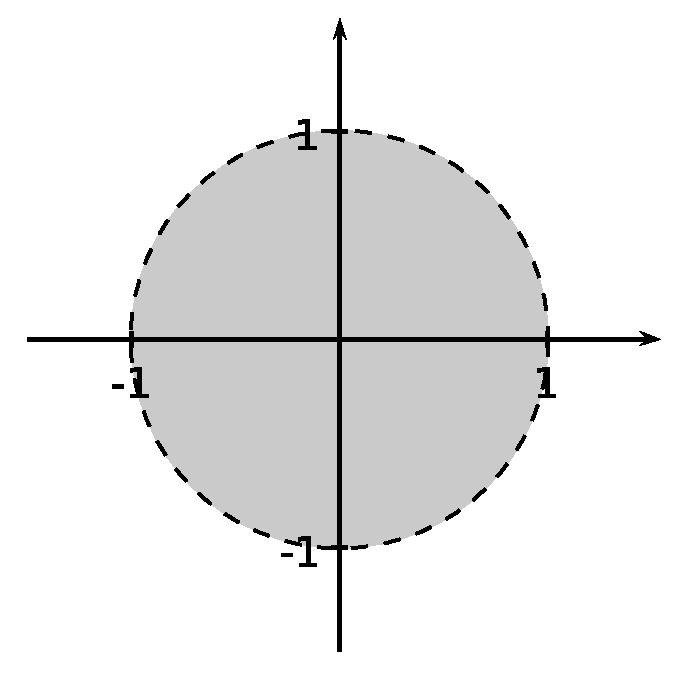
\includegraphics{Rysunki/KulaEuklidesowa}
    }
    % opis obrazka
    \caption[Skr�cony opis do spisu obrazk�w]{Opis pod obrazkiem. Mo�e by� bardzo d�ugi
i zawiera� wiele istotnych informacji. Mo�e m�wi� co przedstawia obrazek, podawa� parametry, wzory
itp.}
    % etykieta
    \label{kula_eulidesowa}
  \end{center}
\end{figure*}


\noindent Po tworzeniu obrazk�w mo�emy je do��czy� w taki spos�b:
\begin{verbatim}
\begin{figure*}[!h]
  % wy�rodkowanie zawarto�ci pola obrazka
  \begin{center}
    % okienko skaluj�ce:
    %  pierwszy argument szeroko��, drugi wysoko��,
    %  jeden z nich mo�e by� zast�piony ! - zachowanie proporcji obrazka
    %  w taki spos�b mo�emy skalowa� tak�e inne obiekty np. tekst
    \resizebox{0.5\textwidth}{!}{
      % wstawienie obrazka
      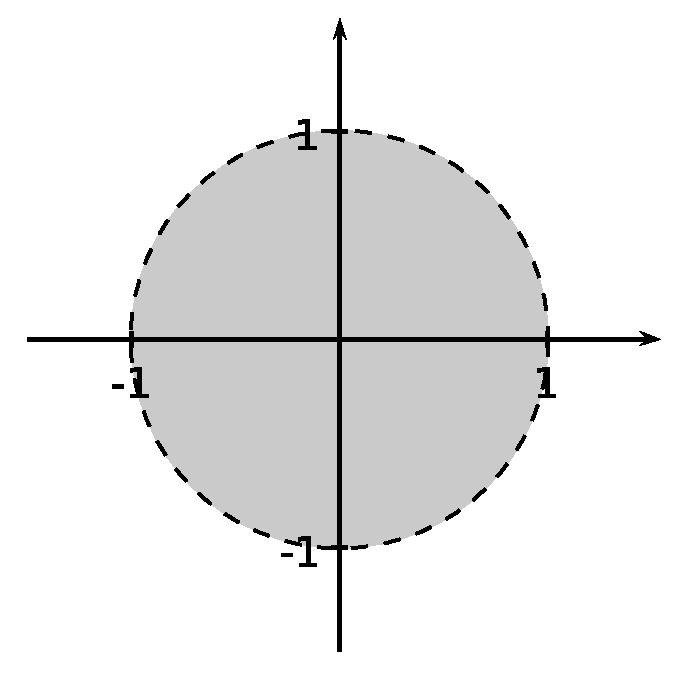
\includegraphics{Rysunki/KulaEuklidesowa}
    }
    % opis obrazka
    \caption[Skr�cony opis do spisu obrazk�w]{Opis pod obrazkiem. Mo�e by� bardzo d�ugi
i zawiera� wiele istotnych informacji. Mo�e m�wi� co przedstawia obrazek, podawa� parametry, wzory
itp.}
    % etykieta
    \label{etykietka_obrazka}
  \end{center}
\end{figure*}
\end{verbatim}

Proponowanym rozwi�zaniem jest tak�e umieszczenie obrazk�w w odr�bnym katalogu znajduj�cym si� w g��wnym folderze pracy dyplomowej. Przyk�adowo w niniejszym szablonie utworzono katalog \verb|rysunki|, z kt�rego do��czy� mo�na obrazek za pomoc� standardowego sposobu pokazanego powy�ej, dodaj�c �cie�k� dost�pu do obrazka np. : 
\begin{verbatim}
\includegraphics[scale=0.5]{rysunki/obrazek1.jpg}
\end{verbatim}


Do obrazk�w mo�emy odwo�ywa� si� u�ywaj�c konstrukcji \verb|\label| -- \verb|\ref|, np.: Rysunek
\ref{kula_eulidesowa} przedstawia kul� w metryce euklidesowej.

\begin{verbatim}
Rysunek \ref{kula_eulidesowa} przedstawia kul� w metryce euklidesowej.
\end{verbatim}

Spis obrazk�w do��czamy do pracy za pomoc� polecenia \verb|\listoffigures|. Sporym problemem mo�e
by� umieszczenie obrazka w konkretnym miejscu na stronie. Je�eli \LaTeX nie potrafi umie�ci�
obrazka tam gdzie chcemy, to mo�e go przenie�� na nast�pn� stron� lub na koniec pliku. Prostym
rozwi�zaniem jest zmiana wielko�ci obrazka. W tym wypadku najlepiej spyta� Google. Og�lna porada
jest taka: pozycjonowanie obrazk�w nale�y wykona� dopiero po napisani ca�ego tekstu, gdy� dodanie
jednej linii tekstu mo�e ca�kowicie zmieni� pozycj� obrazka.

Mo�liwe jest tak�e umieszczenie kilku obrazk�w na jednym rysunku.

\begin{figure*}[!h]
\centering
\subfloat[$X=\mathbb{R}^2$, metryka taks�wkowa]
{
    \resizebox{0.3\textwidth}{!}{
      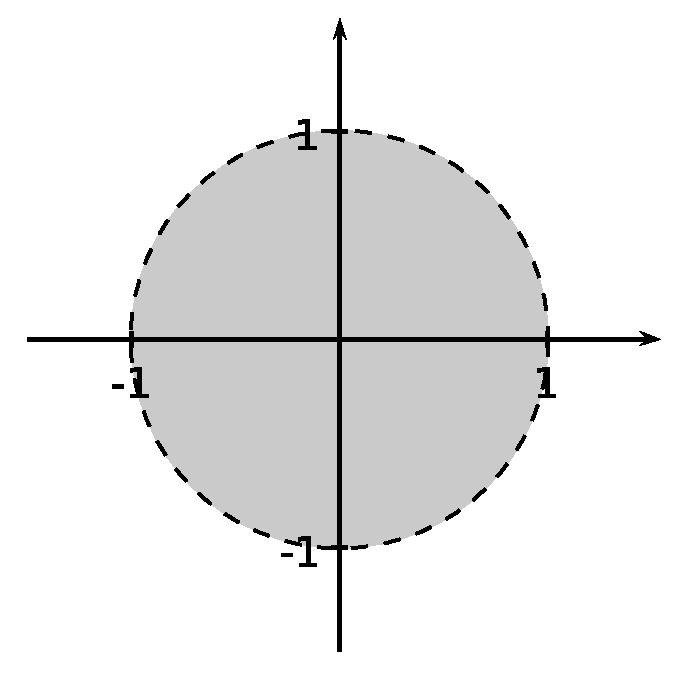
\includegraphics{Rysunki/KulaEuklidesowa}
    }
}
\subfloat[$X=\mathbb{R}^2$, metryka taks�wkowa]
{
    \resizebox{0.3\textwidth}{!}{
      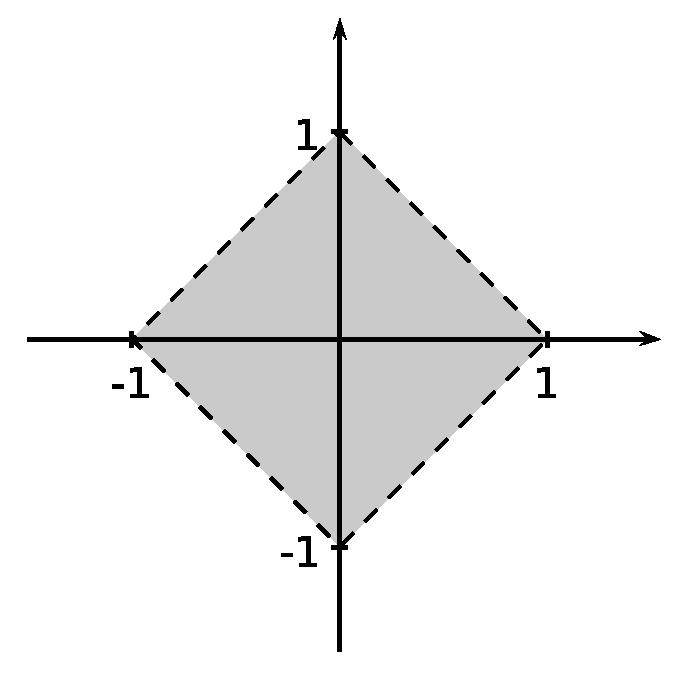
\includegraphics{Rysunki/KulaTaksowkowa}
    }
}
\subfloat[$X=\mathbb{R}^2$, metryka maksimum]
{
    \resizebox{0.3\textwidth}{!}{
      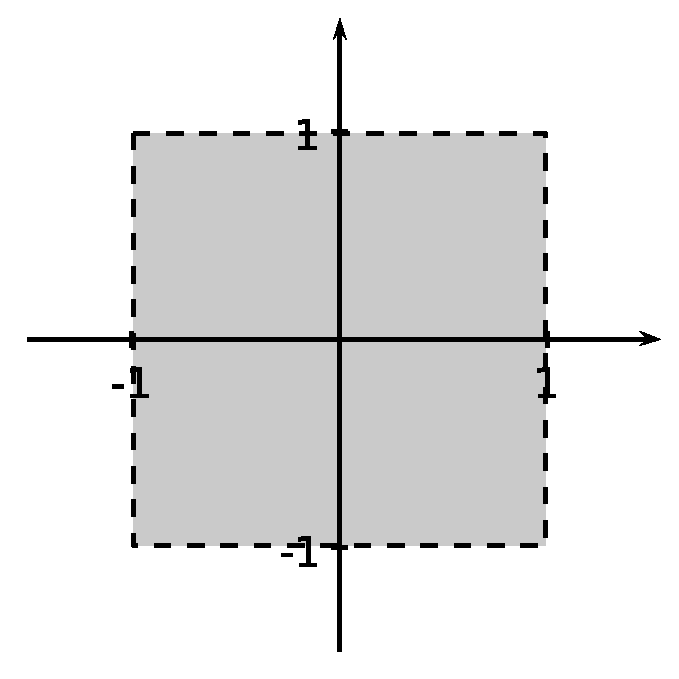
\includegraphics{Rysunki/KulaMaksimum}
    }
}
\caption{Kule w r�nych metrykach}
\end{figure*}

\begin{verbatim}
\begin{figure*}[!b]
\centering
\subfloat[$X=\mathbb{R}^2$, metryka taks�wkowa]
{
    \resizebox{0.3\textwidth}{!}{
      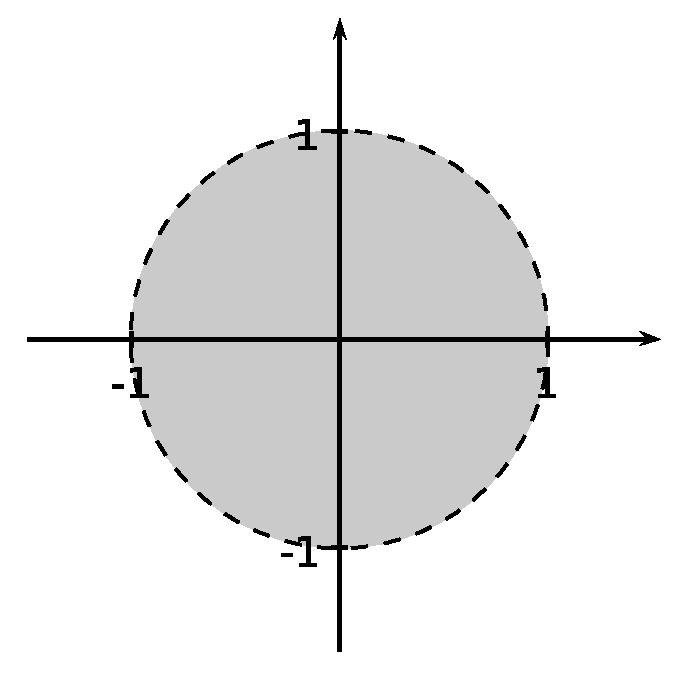
\includegraphics{Rysunki/KulaEuklidesowa}
    }
}
\subfloat[$X=\mathbb{R}^2$, metryka taks�wkowa]
{
    \resizebox{0.3\textwidth}{!}{
      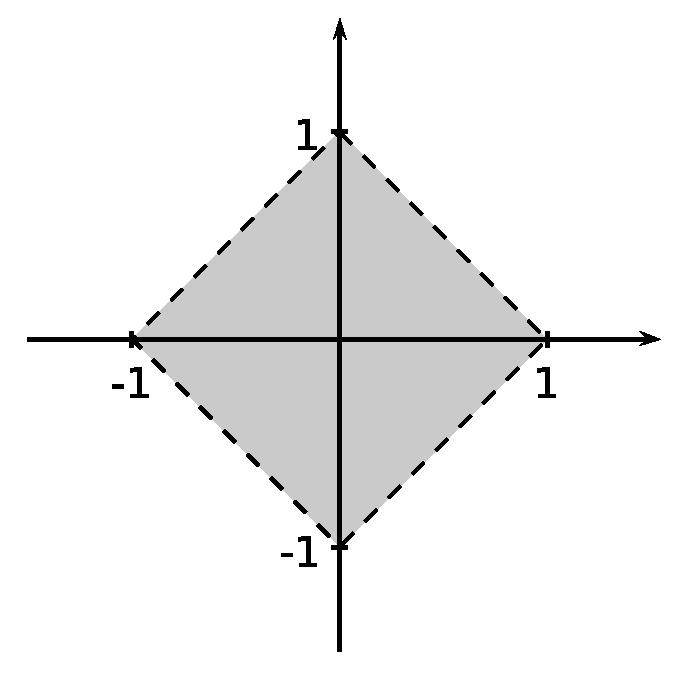
\includegraphics{Rysunki/KulaTaksowkowa}
    }
}
\subfloat[$X=\mathbb{R}^2$, metryka maksimum]
{
    \resizebox{0.3\textwidth}{!}{
      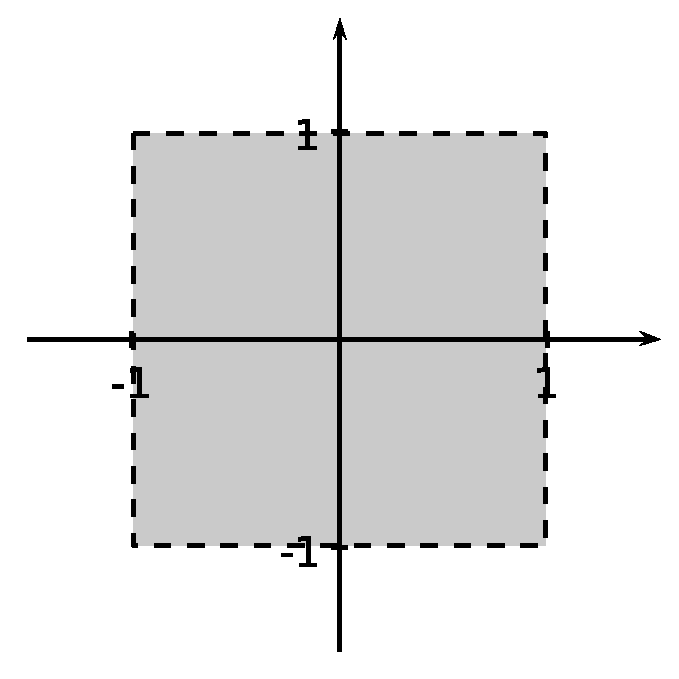
\includegraphics{Rysunki/KulaMaksimum}
    }
}
\caption{Kule w r�nych metrykach}
\end{figure*}
\end{verbatim}


\section{Dodawanie listingu kodu}

W razie potrzeby zamieszczenia listingu kodu omawianego w pracy dyplomowej lub kr�tkich fragment�w tzw. pseudokodu, mo�na wykorzysta� pakiet \verb|listings|. Pakiet ten zawarto w do��czonym do szablonu pakiecie \verb|listing_schemat.sty| kt�ry znajduje si� w g��wnym katalogu. Pakiet ten dodaje si� przez odkometowanie poni�szego polecenia na pocz�tku pliku g��wnego \textbf{SzablonPracyPG\_main.tex}:
\begin{verbatim}
%-------------------- Dodatkowe pakiety ---------------------
\usepackage{listing_schemat}
%------------------------------------------------------------
\end{verbatim}

Przyk�ad  zamieszczenia listingu kodu w pracy przedstawiono poni�ej.
\begin{verbatim}
\lstset{style=python}
\begin{lstlisting}[caption={Przyk�adowy listing w j�zyku Python}, label=pyton]
%%%%%%% KOD �R�D�OWY %%%%%%%
#importing the time module
import time
#welcoming the user
name = raw_input("What is your name? ")
print "Hello, " + name, "Time to play hangman!"
#wait for 1 second
time.sleep(1)
%%%%%%%%%%%%%%%%%%%%%%%%%%%%
\end{lstlisting}
\end{verbatim}

Po skompilowaniu, otrzymuje si� listing w postaci przedstawionej poni�ej.
\lstset{style=python}
\begin{lstlisting}[caption={Przyk�adowy listing w j�zyku Python}, label=pyton]
#importing the time module
import time
#welcoming the user
name = raw_input("What is your name? ")
print "Hello, " + name, "Time to play hangman!"
#wait for 1 second
time.sleep(1)
\end{lstlisting}

Wstawienie listingu rozpoczyna si� poleceniem \verb|\lstset{style=NAZWA_J�ZYKA}|, kt�re ustawia okre�lony spos�b formatowania listingu zale�nie od wybranego j�zyka. Nazw� j�zyka nale�y wpisa� ma�ymi literami. Opracowane formaty j�zyk�w znajduj� si� w pliku pakietu \textbf{listing\_schemat}. Nast�pnie do polecenia \verb|\begin{listings}| podaje si� argumenty wej�ciowe w kwadratowych nawiasach, co przedstawione zosta�o poni�ej. 
\begin{verbatim}
\begin{lstlisting}[caption={Podpis wstawianego listingu}, label=Odno�nik do listingu]
\end{lstlisting}
\end{verbatim}
Podanie wymienionych argument�w wej�ciowych umo�liwia podpisywanie poszczeg�lnych listing�w oraz odwo�ywanie si� do nich w tek�cie przy u�yciu polecenia \verb|\ref{}|.

Istnieje tak�e mo�liwo�� do��czania kodu �r�d�owego, kt�ry zosta� zapisany w osobnym pliku. W tym celu nale�y u�y� poni�szego polecenia.
\begin{verbatim}
\begin{lstlisting}[caption={Podpis wstawianego listingu}, label=Odno�nik do listingu]
\lstinputlisting[language=Python, firstline=10, lastline=20]{plik_zrodlowy.py}
\end{lstlisting}

\end{verbatim}

W pliku pakietu \textbf{listing\_schemat.sty} mo�na zdefiniowa� w�asny styl formatowania listingu, zgodny z u�ywanym j�zykiem programowania. Parametry stylu formatowania zosta�y opisane w pliku, co umo�liwia r�wnie� ewentualn� zmian� kolor�w sk�adni kodu lub innych atrybut�w.

Do pakietu do��czono r�wnie� �rodowisko \verb|tikz|, kt�re umo�liwia generowanie przejrzystych schemat�w blokowych, graf�w, diagram�w oraz wykres�w. Tworzenie diagram�w poprzez opracowanie kodu w edytorze tekstu mo�e by� uci��liwe, jednak istniej� graficzne generatory kodu np. \textbf{TikzEdt} dost�pny pod adresem: \textbf{http://www.tikzedt.org/}.

\section{Dodawanie bibliografii}

Bibliografi� dodajemy za pomoc� nast�puj�cych polece�

\begin{verbatim}
\bibliographystyle{plain}                       % styl bibliografii
\begin{thebibliography}{3}                      % pocz�tek �rodowiska
\addcontentsline{toc}{chapter}{Bibliografia}    % dodaje bibliografi� do spisu tre�ci
\small              % spisy i bibliografie sk�adamy mniejszym stopniem pisma
% przyk�adowy wpis
    \bibitem{Duda}      % \bibitem{etykieta}
A. Duda,\emph{Wprowadzenie do topologii}, PWN, Warszawa 1986
% nast�pna pozycja
    \bibitem{EngeSiek}
R. Engelking, K. Sieklucki, \emph{Geometria i topologia. Cz�� II. Topologia}, PWN, Warszawa 1980
% nast�pna pozycja
    \bibitem{Patk}
H. Patkowska, \emph{Wst�p do topologii}, PWN, Warszawa 1979
% nast�pna pozycja
    \bibitem{Siek}
K. Sieklucki, \emph{Geometria i topologia. Cz�� I. Geometria}, PWN, Warszawa 1979
% nast�pna pozycja
    \bibitem{Rutkowski}
Rutkowski J., \emph{Algebra Abstrakcyjna w zadaniach},  Wydawnictwo Naukowe PWN, Warszawa 2005
\end{thebibliography}                           % koniec �rodowiska
\end{verbatim}

Do pozycji bibliograficznych mo�emy odwo�ywa� si� w tek�cie korzystaj�c z polecenia \verb|\cite|,
np.: G��wnym �r�d�em jest ksi��ka A. Dudy \cite{Duda}. Przyk�ady podane w tym rozdziale pochodz� z
ksi��ki \cite{Rutkowski}.

\begin{verbatim}
G��wnym �r�d�em jest ksi��ka A. Dudy \cite{Duda}.
Przyk�ady podane w tym rozdziale pochodz� z ksi��ki \cite{Rutkowski}.
\end{verbatim}

\section{Uwagi o typografii}

W polskiej typografii (i nie tylko w polskiej) przyj�o si� stosowa� nast�puj�ce zasady:
\begin{itemize}
    \item na ko�cu wiersza nie mog� zosta� s�owa jednoliterowe (dwu-, trzy-) (tzw. sierota)
    \item akapit nie mo�e ko�czy� si� bardzo kr�tkim wierszem: pojedyncze s�owo, przeniesiona
cz�� s�owa lub kr�tkich s��w, orientacyjnie, mniej ni� 3 d�ugo�ci wci�cia akapitowego (tzw. wdowa)
\tiny{<-- wdowa}\normalsize
    \item strona nie mo�e ko�czy� si� pojedynczym wierszem nowego akapitu (tzw. szewc)
    \item strona nie mo�e zaczyna� si� ostatnim wierszem poprzedniego akapitu (tzw. b�kart)
    \item unika� podw�jnych wyr�nie�, nie nale�y wyr�nianego fragmentu tekstu wyr�nia� wi�cej ni�
jedn� metod� naraz (np.: \textbf{\textit{podw�jne wyr�nienie}})
\begin{verbatim}
https://pl.wikipedia.org/wiki/Zasada_unikania_podw�jnych_wyr�nie�
\end{verbatim}
\end{itemize}

Niestosowanie si� do tych zasad nie umniejsza warto�ci pracy, jednak zmniejsza jej estetyk� a w
przypadku pojedynczych wierszy utrudnia czytanie. W tym dokumencie mo�na znale�� przyk�ady takich
sytuacji.


Aby usun�� wspomniane b��dy zwykle wystarczy zmieni� szyk zdania lub u�y� innego s�owa. W
ostateczno�ci(!) mo�na doda� pusty wiersz. Aby usun�� pojedyncze litery na ko�cu wiersza mo�na
doda� tzw. tward� spacj�, umieszczaj�c pomi�dzy wyrazami znak tyldy \textasciitilde.

\begin{przyklad}
d�ugies�owo i kr�tkie i d�ugies�owo i kr�tkie i d�ugies�owo i kr�tkie i d�ugies�owo i kr�tkie i
d�ugies�owo i kr�tkie i d�ugies�owo i kr�tkie i d�ugies�owo i kr�tkie i d�ugies�owo i kr�tkie i
\end{przyklad}

\begin{przyklad}
d�ugies�owo i kr�tkie i d�ugies�owo i kr�tkie i d�ugies�owo i kr�tkie i d�ugies�owo i~kr�tkie i
d�ugies�owo i kr�tkie i d�ugies�owo i kr�tkie i d�ugies�owo i kr�tkie i d�ugies�owo i kr�tkie i
\end{przyklad}


Podobnie jak w przypadku obrazk�w, poprawki typograficzne powinny by� wprowadzane po zako�czeniu
pisania pracy, gdy� nawet najmniejsza zmiana w poprzednim wierszu mo�e skutkowa� powa�nymi
przesuni�ciami ca�ego tekstu.


Jako ciekawostka: norma PN-83/P-55366 (nieobowi�zuj�ca od kilku lat) podaje seri� wskaz�wek i
zalece� typograficznych.
\chapter{Uwagi od strony technicznej}

\section{Opcje}

\begin{enumerate}
 \item \verb|strict| -- domy�lnie, klasa stara si� jak naj�ci�lej wype�nia� zalecenia
 \item \verb|nostrict| -- drobne modyfikacje typograficzne
 \begin{itemize}
  \item zmniejszenie wci�cia akapitowego z 1.25cm na 1.5em
 \end{itemize}
\end{enumerate}

\section{Wymagane pakiety}
Lista pakiet�w, kt�re s� wymagane do kompilacji (wi�kszo�� z nich jest zapewne zainstalowana
domy�lnie)
\begin{enumerate}
  \item \verb|polski| -- polonizacja \TeX'a
  \item \verb|fontenc| -- kodowanie znak�w
  \item \verb|inputenc| -- kodowanie znak�w
  \item \verb|helvet| -- wybiera font podobny do Arial
  \item \verb|geometry| -- ustawienie margines�w
  \item \verb|indentfirst| -- wci�cie pierwszego akapitu
  \item \verb|fancyhdr| -- paginacja
  \item \verb|titlesec| -- tytularia
  \item \verb|titletoc| -- formatowanie spisu tre�ci
  \item \verb|enumitem| -- wyliczenia numerowane i nienumerowane
  \item \verb|amsmath,amssymb,amsthm| -- standardowe pakiety matematyczne
  \item \verb|graphicx| -- do��czanie obrazk�w
  \item \verb|subfig| -- wiele obrazk�w na jednym rysunku
  \item \verb|caption| -- format podpisu pod obrazkiem
  \item \verb|tikz| -- generowanie schemat�w blokowych i innych rysunk�w
  \item \verb|listings| -- umieszczanie listing�w kodu w pracy
\end{enumerate}

\section{Fonty}

Wymaganym fontem jest Arial. Poniewa� taki font nie jest �atwo dost�pny w \LaTeX'u wi�c korzystamy
z fonta zast�pczego w pakiecie \verb|helv|. Wymagany font matematyczny nie zosta� podany. U�ywamy
zatem fontu z pakietu \verb|mathpazo|.
\begin{verbatim}
\usepackage{helvet}
\usepackage{mathpazo}
\renewcommand{\familydefault}{\sfdefault}
\end{verbatim}

Inn� wersje fontu bezszeryfowego mo�na uzyska� poprzez zrezygnowanie z pakietu \verb|helv|.

Przyk�adowy: $\sin(x)+ay^2$.
\[
 \sin(x)+ay^2
\]



% ---------------------- Bibliografia -----------------------
\bibliographystyle{plain}                       % styl bibliografii
\begin{thebibliography}{3}                      % pocz�tek �rodowiska
\addcontentsline{toc}{chapter}{Wykaz literatury}    % dodaje bibliografi� do spisu tre�ci

\small              % spisy i bibliografie sk�adamy mniejszym stopniem pisma
% przyk�adowy wpis
    \bibitem{BiznesRadar.pl}      % \bibitem{etykieta}
BiznesRadar.pl 
% nast�pna pozycja
    \bibitem{Kahn}
Michael N. Kahn: \emph{Analiza techniczna}, wyd. GAB, 2018
% nast�pna pozycja
    \bibitem{Majchrowski}
Dr Klaudiusz Majchrowski: \emph{Wyk�ad dla Elekroradiologii, Podstawy elektroniki i akustyki}, www.ur.edu.pl/file/71671/Podstawy
% nast�pna pozycja
    \bibitem{Wiki_sygnal}
Wikipedia: \emph{Sygna�}, pl.wikipedia.org/wiki/Sygna\%C5\%82\#Zastosowania
% nast�pna pozycja
    \bibitem{Erhard}
Jan Erhard: \emph{Technika cyfrowa - podstawy}, www.livesound.pl/tutoriale/3938-technika-cyfrowa-podstawy.-zacznijmy-od-poczatku.
% nast�pna pozycja
    \bibitem{lomiowka}
Szko�a w Mil�wce: \emph{Zapis analogowy i cyfrowy d�wi�ku}, www.lomilowka.pl/pliki/1\_zapis\_dzwieku\_pdf-9092.pdf
% nast�pna pozycja
    \bibitem{wiki_dyskretyzacja}
Wikipedia: \emph{Dyskretyzacja}, pl.wikipedia.org/wiki/Dyskretyzacja\_(statystyka)
% nast�pna pozycja
    \bibitem{wiki_kwantyzacja}
Wikipedia: \emph{Kwantyzacja}, pl.wikipedia.org/wiki/Kwantyzacja\_(technika)\#Kwantyzacja\_sygna\%C5\%82u\_analogowego
% nast�pna pozycja
    \bibitem{Labaj}
Weronika �abaj: \emph{Sygna�}, zasoby.open.agh.edu.pl/~10swlabaj/sygnal/sygnal2.html
% nast�pna pozycja
    \bibitem{Jozwiak}
Arkadiusz J�wiak: \emph{3 sposoby jak wykorzysta� �rednie krocz�ce}, comparic.pl/3-sposoby-wykorzystac-srednie-kroczace-tradingu/
% nast�pna pozycja
    \bibitem{edukacja_gieldowa}
Strona edukacja gie�dowa: \emph{Analiza techniczna}, www.edukacjagieldowa.pl/gieldowe-abc/analiza-techniczna/
% nast�pna pozycja
    \bibitem{Google_Play}
Google Play: \emph{Aplikacja BiznesRadar}, play.google.com/store/apps/details?id=com.Android.BiznesRadar\&hl=pl
% nast�pna pozycja
    \bibitem{tradersarea}
Strona tradersarea: \emph{MACD jako jeden z najpopularniejszych wska�nik�w}, tradersarea.pl/macd-jako-jeden-z-najpopularniejszych-wskaznikow/
% nast�pna pozycja
    \bibitem{edu_gield_macd}
Strona edukacja gie�dowa: \emph{Krzywa MACD}, https://www.edukacjagieldowa.pl/gieldowe-abc/analiza-techniczna/narzedzia-analizy-technicznej/krzywa-macd/
% nast�pna pozycja
    \bibitem{TradingView}
Strona TradingView: \emph{MACD, zbie�no��/ rozbie�no�� �rednich ruchomych}, www.tradingview.com/wiki/MACD\_(Moving\_Average\_Convergence/Divergence)/pl
% nast�pna pozycja
    \bibitem{admiralmarkets}
Strona admiralmarkets: \emph{Wska�nik MACD - najpopularniejszy ze wska�nik�w}, https://admiralmarkets.pl/education/articles/forex-indicators/wskaznik-macd
% nast�pna pozycja
    \bibitem{stooq}
Serwis stooq: www.stooq.pl
% nast�pna pozycja
    \bibitem{edu_gield_stoch}
Strona edukacja gie�dowa: \emph{Oscylator stochastyczny}, www.edukacjagieldowa.pl/gieldowe-abc/analiza-techniczna/narzedzia-analizy-technicznej/oscylator-stochastyczny/
% nast�pna pozycja
    \bibitem{admiralmarkets_stoch}
Strona admiralmarkets: \emph{Oscylator Stochastyczny - Handel w Oparciu o Stochastic}, admiralmarkets.pl/education/articles/forex-indicators/oscylator-stochastyczny
% nast�pna pozycja
    \bibitem{tradersarea_stoch}
Strona tradersarea: \emph{Oscylator Stochastyczny Stochastic}, tradersarea.pl/oscylator-stochastyczny-stochastic/
% nast�pna pozycja
    \bibitem{zielinski}
Tomasz P. Zieli�ski: \emph{Cyfrowe przetwarzanie sygna��w}, wyd. Komunikacji i ��czno�ci sp. z.o.o Warszawa 2005, 2009
% nast�pna pozycja
    \bibitem{numba}
Numba: \emph{installation}, numba.pydata.org/numba-doc/dev/user/installing.html
% nast�pna pozycja
    \bibitem{rpubs_installation}
Mohammad Shadan: \emph{Python - Install Anaconda, Jupyter Notebook}, rpubs.com/mohammadshadan/installanaconda
\vspace{0.8cm} \\
Wszystkie adresy stron www s� aktualne na dzie� 01.12.2019r.
\end{thebibliography}                           % koniec �rodowiska % dodanie pliku bibliografii
% -----------------------------------------------------------

%------------------------------------------------------------
%	Dodanie wykazu rysunk�w oraz tabeli

\renewcommand{\baselinestretch}{1.0}\normalsize	% interlinia w sekcji wykaz�w
\addcontentsline{toc}{chapter}{\listfigurename}	% dodanie wykazu rysunk�w do spisu tre�ci
\listoffigures									% generacja wykazu rysunk�w

\addcontentsline{toc}{chapter}{\listtablename}	% dodanie wykazu tabel do spisu tre�ci
\listoftables									% generacja wykazu tabel
\renewcommand{\baselinestretch}{1.3}\normalsize	% powr�t do interlinii 1.5


% -----------------------------------------------------------
\end{document}
%------------------------------------------------------------
			 			%	Koniec   %
%------------------------------------------------------------
